\section{Η προσέγγισή μας}\label{our_approach}

Η προσέγγισή μας έχει 3 βασικά μέρη:
\begin{itemize}
	\item \textbf{Κατάτμηση} των PCG δειγμάτων στις βασικές περιοχές του καρδιακού
	      ήχου.
	\item \textbf{MFCC μετασχηματισμό} των PCG δειγμάτων σε αναπαράσταση
	      χρόνου-συχνότητας της κατανομής της ενέργειας του σήματος.
	\item \textbf{Εκπαίδευση \& Κατηγοροποίηση} των MFCC heat maps με την χρήση
	      του συνελικτικού νευρωνικού δικτύου.
\end{itemize}

\subsection{Κατάτμηση Δειγμάτων}

Για να κάνουμε την κατάτμηση των PCG δειγμάτων όπως φαίνεται στην εικόνα
\ref{PCG} θα χρησιμοποιήσουμε των αλγόριθμο του Springer
\cite{springer2015logistic} τον οποίο τον παρείχε ο διαγωνισμός στους
συμμετέχοντες. Ωστόσο δεν θα χρησιμοποιήσουμε όλα τα δεδομένα που μας δίνει ο
αλγόριθμος, αλλά αυτό που θα κάνουμε είναι να βρίσκουμε που ξεκινάει το πρώτο
\emph{S1} και στη συνέχεια θα αναλύουμε τα 3 επόμενα δευτερόλεπτα. Αυτή η
διαδικασία θα γίνεται ώστε τα δείγματα με τα οποία θα εκπαιδεύσουμε το νευρονικό
δίκτυο να είναι ``ευθυγραμισμένα'' μεταξύ τους.


\subsection{Μετασχησματισμός MFCC}

Αφού πάρουμε τα 3 δευτερόλεπτα σκοπός είναι να δημιουργήσουμε μια εικόνα που θα
απεικονίζει χαρακτηριστικά του ηχητικού αποσπάσματος ώστε να μπορέσουμε να
προπονήσουμε το νευρωνικό μας δίκτυο. Αυτό μπορούμε να το πετύχουμε
υπολογίζοντας τις MFCC τιμές του καρδιογραφήματος με την εξής διαδικασία:

\begin{enumerate}
	\item Παίρνουμε επικαλυπτόμενα παράθυρα πάνω στο ηχητικό δείγμα
	\item Υπολογίζουμε τον μετασχηματισμό Fourier για κάθε παράθυρο
	\item Εφαρμόζουμε τα Mel φίλτρα και αθροίζουμε τις ενέργειες σε κάθε φίλτρο
	\item Υπολογίζουμε τις λογαριθμικές τιμές των παραπάνω ενεργειών
	\item Τέλος παίρνουμε τον διακριτό συνημιτονικό μετασχηματισμό των λογαριθμικών
	      τιμών.
\end{enumerate}

Έτσι θα έχουμε 12 MFCC τιμές για κάθε παράθυρο και μαζί με την ολική ενέργεια
του παραθύρου ως ξεχωριστή τιμή παίρνουμε 13 τιμές. Αναπαριστώντας αυτά τα
χαρακτηριστικά σε ένα γράφημα όπου ο $y$ άξονας θα κυμαίνετε από 0 εώς 12 (μία
γραμμή για κάθε MFCC τιμή) και ο $x$ άξονας από 0 εώς $3000 / step\_size$
(\emph{step\_size} που θα ορίσουμε για κάθε παράθυρο), θα πάρουμε ένα heat map
(βλέπε \ref{mfcc}) που μπορούμε να χρησιμοποιήσουμε ως εικόνα για το νευρωνικό
δίκτυο.

\begin{figure}[H]
	\center
	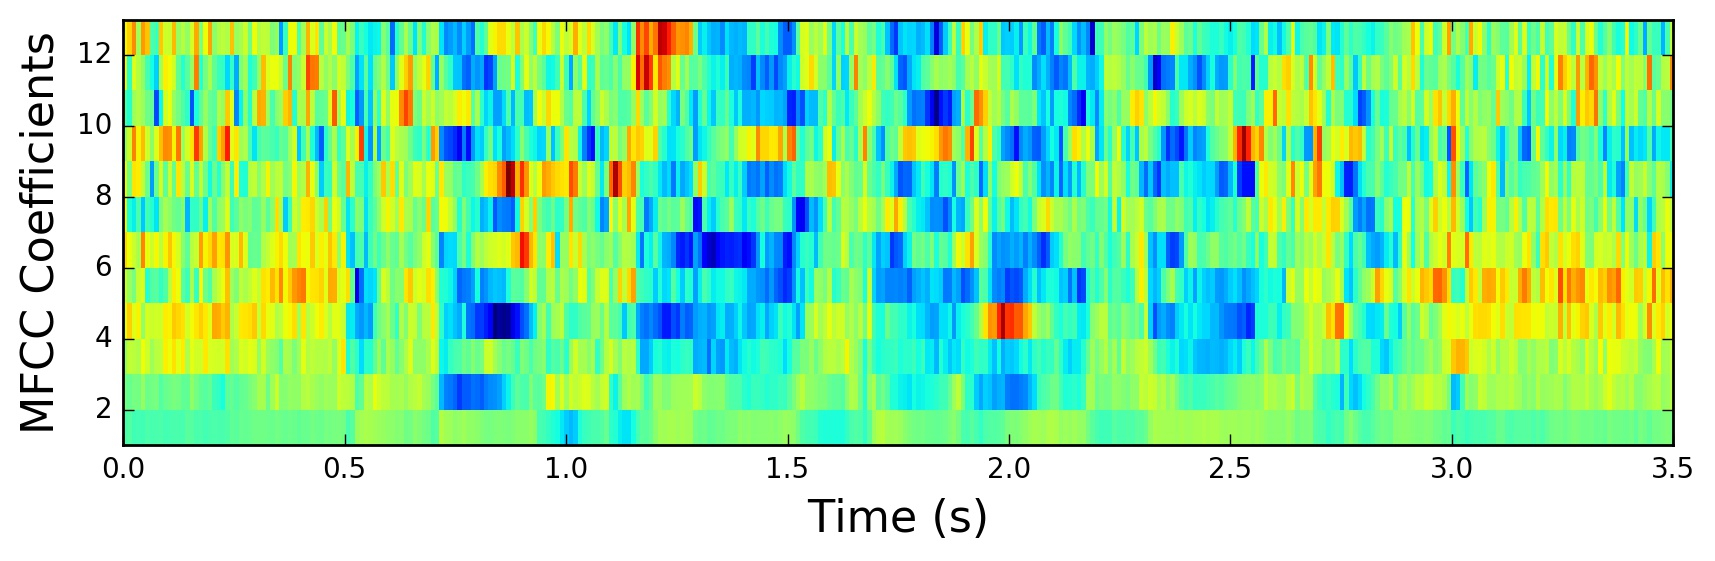
\includegraphics[width=0.7\textwidth]{mfcc.jpeg}
	\caption{MFCC heat map \cite{fayek2016}}
	\label{mfcc}
\end{figure}

\subsection{Νευρωνικό δίκτυο}

Η μετατροπή των δοθέντων μονοδιάστατων χρονοσειρών σε πίνακες θερμότητας δύο διαστάσεων
μας επιτρέπει την επεξεργασία δειγμάτων των καρδιακών ήχων υπό τη μορφή εικόνας. Γι' αυτό
κρίνεται και επιβεβλημένη η χρήση συνελικτικών νευρωνικών δικτύων λόγω των αυξανόμενων
δυνατοτήτων τους στην ανάλυση εικόνων.
\subsubsection{Αρχιτεκτονική δικτύου}

Το νευρωνικό δίκτυο δέχεται σαν είσοδο ένα κανάλι 13x300 MFCC χάρτη θερμότητας
(αν χρησιμοποιήσουμε βήμα 10ms στον MFCC μετασχηματισμό) και δίνει σαν τελική
έξοδο την ζητούμενη δυαδική κατηγοριοποίηση. Ενδιάμεσα χρησιμοποιούνται δύο
συνελικτικά στρώματα, το καθένα ακολουθούμενο από ένα στρώμα max-pooling, και
συνολικά ακολουθούμενο από δύο πλήρως συνδεδεμένα κρυφά στρώματα. \par

Το πρώτο συνελικτικό στρώμα μαθαίνει 64 2x20 πυρήνες,χρησιμοποιώντας την τεχνική
same-padding.  Στη συνέχεια εφαρμόζουμε ένα max-pooling φίλτρο
1x20,χρησιμοποιώντας ένα οριζόντιο βήμα μήκους 5, το οποίο έχει ως αποτέλεσμα τη
μείωση των διαστάσεων καθενός από τους 64 χάρτες χαρακτηριστικών σε 13x60. Ένα
δεύτερο συνελικτικό στρώμα χρησιμοποιεί 64 πυρήνες 2x10 επάνω στο προηγούμενο
στρώμα,ξανά με same-padding.Μετά την προαναφερθείσα διαδικασία ακολουθεί και
πάλι η διαδικασία max-pooling,με την χρήση φίλτρου 1x4 και βήματος 2,μειώνοντας
με αυτό τον τρόπο τη διάσταση του χάρτη χαρακτηριστικών σε 13x30.Ακολουθεί μια
διαδικασία πλάτυνσης για την μετατροπή καθενός από τους 64 13x30 χάρτες
χαρακτηριστικών σε διάνυσμα μεγέθους 24,960. Το διάνυσμα αυτό εισάγεται στο
πρώτο πλήρως συνδεδεμένο κρυφό στρώμα μήκους 1024 κρυφών μονάδων
και,ακολουθούμενο από ένα δεύτερο κρυφό στρώμα 512 κρυφών μονάδων,δίνει την
δυαδική έξοδο κατηγοριοποίησης. \par

\begin{figure}[H]
	\center
	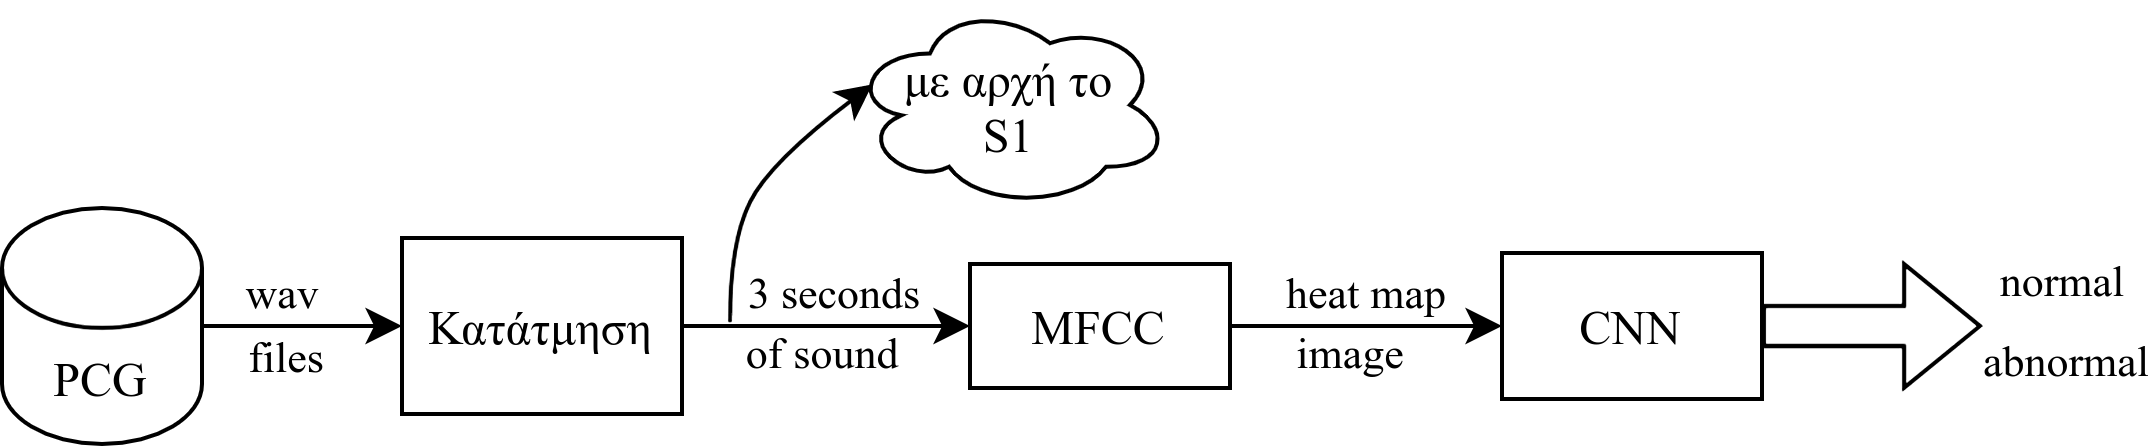
\includegraphics[width=\textwidth]{hear_sound_classification_diagram.png}
	\caption{Διάγραμμα της προσέγγισής μας για την κατηγοροποίηση καρδικών ήχων}
	\label{our_approach_diagram}
\end{figure}
